\chapter{Trigger Logic and Data Taking}
\label{sec:trigger}
The trigger system is a logic circuit that can select muons
that do not cross the setup. So, we can retrieve a signal of a stopping muon 
that can be used as a start signal for the time measurement of the decay.
If we take \autoref{fig:Setup} as a reference of the experimental apparatus, 
each of the half-planes of plane 0 has two PMTs, connected with an AND gate.
The two half-planes with an OR gate in this way, only the signal
that activate the two PMTs can enter the circuit as shown in \autoref{fig:logig_plane0}.
By doing this, we avoid detecting too much background.
Meanwhile, the OR gate is needed since there are two half-planes
and a muon can cross either two.\\
\begin{figure}[h]
\begin{center}
\includegraphics[width=80 mm,scale=0.5]{figures/Cattura2.png}
\end{center}
\caption{Logic circuit of plane 0.}
\label{fig:logig_plane0}
\end{figure}
We repeat the process for plane 1. For plane 2, we want a NOT gate at the end of the OR gate, so that we have a signal when no muons cross P2 to make sure that the muon has actually stopped. The P0, P1 and NOT P2 will be connected to an AND
gate so that only when all of them generate a signal, we can have the Trigger signal as
shown in \autoref{fig:trigger_system}.

\begin{figure}[h]
\begin{center}
\includegraphics[width=100mm]{figures/Cattura3.png}
\end{center}
\caption{Trigger system.}
\label{fig:trigger_system}
\end{figure}

For the time measurement, we use a couple of TDCs in series since we need a least 10$\;\symup{\mu}$s
and the max time measurable for this TDC is 5$\;\symup{\mu}$s.
The TDC is controlled by a crate controller that sends the information 
from the module. The crate controller works with a DAQ code (labVIEW) 
that creates a memory location that will be read by the crate, which will give a command to the
CAMAC module in this way
\begin{enumerate}
  \item If and only 1 of the clock of the TDC has a stop before the time limit (5$\;\symup{\mu}$s), then a memory location called LAM, is set to 1
  \item The crate reads the memory location of the LAM continuously; if it is 1 the create controller stops the reading, the LAM reads the measurement and clears them to start again
\end{enumerate}
 If there is no stopping signal in the 5$\;\symup{\mu}$s time limit, the LAM will never be set to 1, so the crate controller will never stop the measurement and clear the memory leading to the DAQ problem. We can solve this by taking a copy of the start signal, delaying it by 4.7$\;\symup{\mu}$s and connecting it to one of the clocks of the TDC in this way, so we have
a fake stop that will set the LAM to 1 to prevent the problem. With this in mind, we build the circuit shown in \autoref{fig:daq}.\\
\begin{figure}[h]
\begin{center}
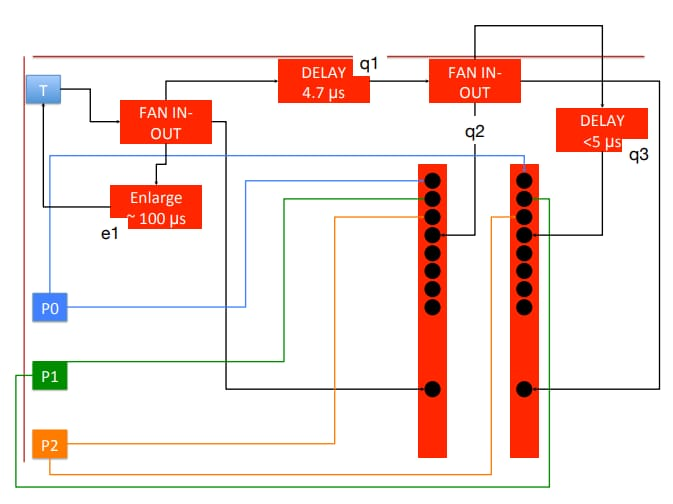
\includegraphics[width=100mm]{figures/cattura4.png}
\end{center}
\caption{Data acquisition circuit.}
\label{fig:daq}
\end{figure}

The first three clocks would be connected to the P0, P1 and P2 in search of an electron
appearence signal. The start, for the first TDC, is given by the trigger, and then we take a copy
of it and delay it by 4.7$\;\symup{\mu}$s (q1). From this, we take three copies with a fan-in-fan-out :
\begin{enumerate}
\item the first will be used as the fake stop for the first TDC (q2)
\item the second will be the start of the second TDC
\item the third will be delayed again by a time $<5\;\symup{\mu}$s and used as a fake stop for the second TDC (q3)
\end{enumerate}
The last thing is to make sure that no trigger is generated in the deadtime of the DAQ, so we take the signal, enlarge it up to 100$\;\symup{\mu}$s, and send it back to the logic unit that provides the trigger in the VETO input (e1).\\
